La seconde partie du processus de \emph{spatialisation} est le
\emph{calcul de la métrique.} C'est durant cette phase qu'est calculée
la mesure utilisée pour quantifier une grandeur que l'on veut
représentative de la sémantique de la \emph{relation de localisation
  atomique} \emph{spatialisée.} Les \emph{métriques} sont plus
nombreuses et diverses que les \emph{rasterisers.}

\subsection{Classification}

Le concept de \enquote{\emph{métrique}} est assez vaste et de
nombreuses XXX 

Les \emph{métriques} que nous sommes amenés à construire peuvent être
de nature et porter sur ds phénomènes assez différents. Toutefois on
peut identifier une certaine récurrence dans leurs
caractéristiques.

Tout d'abord certaines \emph{métriques} quantifient des phénomènes
exprimés par rapport à \emph{l'objet de référence.}  C'est par exemple
le cas des matrices 4IM, utilisées précédemment pour introduire la
méthodologie de \emph{spatialisation.} En effet, la valeur de la
matrice calculée en un pixel dépend de la position et de la forme de
\emph{l'objet de référence,} si ce dernier change, la \emph{métrique}
sera caduque. Cependant des \emph{métriques} comme la pente ou
l'altitude, utilisées pour \emph{spatialiser} des \emph{indices de
  localisation} tels que : \enquote{Je suis à \SI{2500}{\meter}} ou
\enquote{Nous sommes dans une zone de forte pente}, ne dépendent pas
d'un \emph{objet de référence.} On parle dans ce cas de
\emph{métriques intrinsèques,} que l'on oppose aux \emph{métriques
  extrinsèques,} telles que la distance à \emph{l'objet de référence}
ou une relation topologique.

Un second critère peut être utilisé pour distinguer les
\emph{métriques.} En effet, certaines d'entre elles nécessitent un
paramétrage pour être calculées. C'est par exemple le cas d'une
\emph{métrique} comme le temps de marche, qu'il est nécessaire de
paramétrer en fonction de la vitesse de déplacement.
%
Il peut cependant être délicat de différentier ce qui est rattaché à
la paramétrisation et ce qui se rattache à la métrique
%
Cependant une
grande partie des \emph{métriques} ne nécessitent pas de paramétrage,
c'est notamment le cas de la distance à \emph{l'objet de référence} ou
de l'altitude, déjà citées.

Ces deux critères se combinent et (\autoref{fig:type_metriques})

\subsection{Les différentes \emph{métriques}}

Parmi tous les exemples que nous avons présentés, une \emph{métrique}
apparait régulièrement, la \emph{distance planimétrique} à
\emph{l'objet de référence} (\autoref{fig:ISO_DIST_HT}). Cette
\emph{métrique} est un exemple caractéristique des \emph{métriques
  extrinsèques} et \emph{non paramétriques.} Il est, en effet,
nécessaire de la calculer pour chaque \emph{objet de référence,} mais
elle n'accepte pas de \emph{paramètres.}  On pourrait cependant en
ajouter, par exemple en ajoutant un paramètre permettant d'employer
des distances alternatives, comme la distance de Manhattan, de
Minkowski ou de Tchebychev. Mais ces distances alternatives, trop
éloignées de la perception humaine des distances, ne présentent pas
d’intérêt pour notre cas d'application. Cette \emph{métrique} est
employée lors de la \emph{spatialisation} de toutes les
\emph{relations de localisation atomiques} traduisant un éloignement
ou une relation topologique.

\begin{table}
  \centering
  \begin{tabular}{>{\bfseries}R{3cm}C{5cm}C{5cm}}
  \toprule
  &
   \multicolumn{1}{c}{\bfseries Paramétriques} &
   \multicolumn{1}{c}{\bfseries Non Paramétriques} \\
  \midrule
  Extrinsèques &&Pente\\
  Intrinsèques &&\\
  \bottomrule
\end{tabular}

  \caption{Types de métriques}
  \label{fig:type_metriques}
\end{table}

Une autre \emph{métrique,} également utilisée lors de la comparaison
des implémentations (\autoref{chap:06}), est la différence d'altitude
entre une position et \emph{l'objet de référence.} Il s'agit une
nouvelle fois d'une \emph{métrique extrinsèque} et \emph{non
  paramétrique.} 

\begin{figure}
  \centering
  \begin{tikzpicture}
  \tikzset{et/.style={above,font=\footnotesize\vphantom{Ag}}}
  %
  \node[inner sep=0pt, anchor=south west] (image) at (0,0){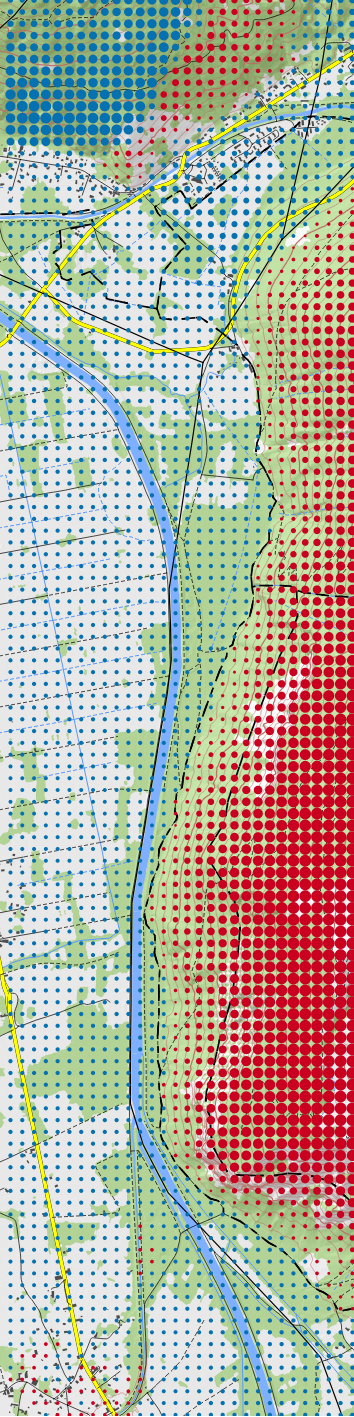
\includegraphics[angle=90]{./figures/Metrique_delta_alt.png}};
  %
  \begin{scope}
    \node (P2) at ([yshift=-.5cm]image.south east) {};
    \node (P1) at ([yshift=-.5cm]image.south west) {};
    %
    \foreach \x [evaluate=\xshift using \x/10, evaluate=\rad using (\x * .0004) + .01] in {0,...,100}
    {
      \draw[fill=black,draw=none, below] ([xshift=\xshift cm, yshift=-.5cm]P1) circle [radius=\rad cm];
    }
    %
    \path(P1 |- 0cm,-1cm) --++ (10,0)
    node[et,pos=0] {0}
    node[et,pos=.1] {0,1}
    node[et,pos=.2] {0,2}
    node[et,pos=.3] {0,3}
    node[et,pos=.4] {0,4}
    node[et,pos=.65] {0,65}
    node[et,pos=1] {1};
    % Échelle
    \draw[-] (P2 |- -1cm,-1cm) --++ (-1,0) node[et,pos=.5] {\SI{500}{\meter}};
    % Légende détaillée
    \path (P1) -- (P2) node[pos=.5, yshift=-1cm] {\tiny Pour la légende détaillée du fond topographique voir \autoref{anx:topo_leg}. Sources: BD TOPO 2018, BD ALTI 2018.}; 
  \end{scope}
\end{tikzpicture}
  \caption{Métrique 2 À  changer ??}
\end{figure}

Pour \emph{spatialiser} les \emph{relations de localisation atomiques}
XXX aux angles, deux \emph{métriques} ont été développées,
\onto{Ecart\-Angulaire} et \onto{Direction\-De}. Toutes deux sont des
\emph{métriques} extrinsèques et paramétriques. La \emph{métrique}
\onto{Ecart\-Angulaire} est destinée à mesurer l'écart à une
orientation donnée.
%
(\autoref{fig:metrique_ecart_angulaire})

\begin{figure}
  \centering
  \begin{tikzpicture}
  \tikzset{et/.style={above,font=\footnotesize\vphantom{Ag}}}
  %
  \node[inner sep=0pt, anchor=south west] (image) at (0,0){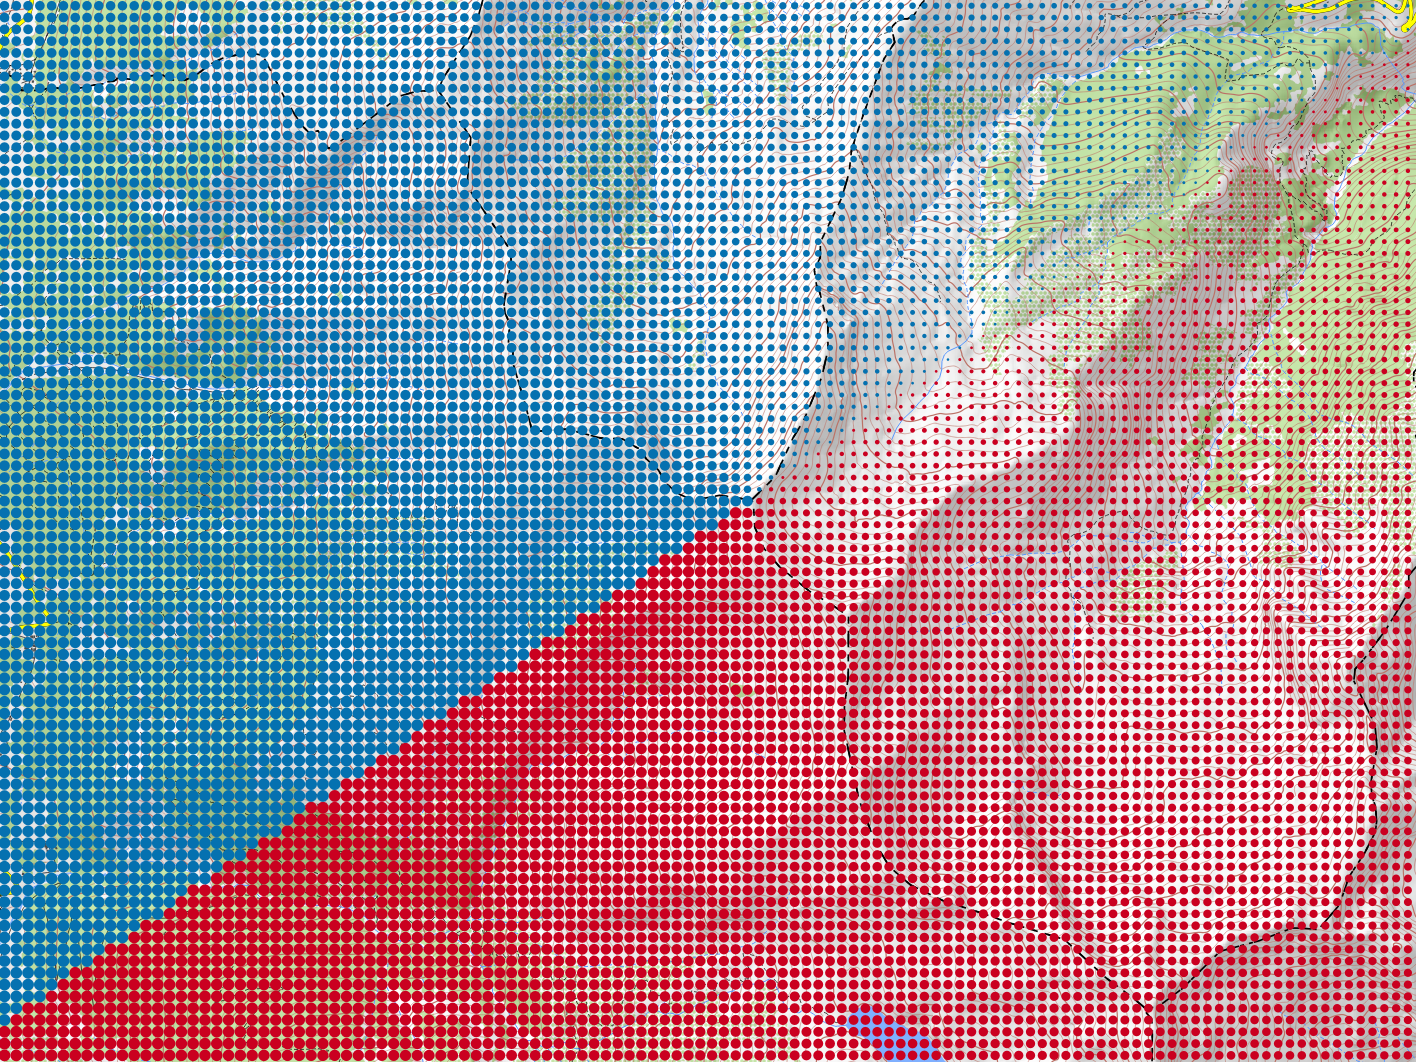
\includegraphics{./figures/Metrique_ecart_valeur.png}};
  %
  \begin{scope}
    \node (P2) at ([yshift=-.5cm]image.south east) {};
    \node (P1) at ([yshift=-.5cm]image.south west) {};
    %
    \foreach \x [evaluate=\xshift using \x/10, evaluate=\rad using (\x * .0004) + .01] in {0,...,100}
    {
      \draw[fill=black,draw=none, below] ([xshift=\xshift cm, yshift=-.5cm]P1) circle [radius=\rad cm];
    }
    %
    \path(P1 |- 0cm,-1cm) --++ (10,0)
    node[et,pos=0] {0}
    node[et,pos=.1] {0,1}
    node[et,pos=.2] {0,2}
    node[et,pos=.3] {0,3}
    node[et,pos=.4] {0,4}
    node[et,pos=.65] {0,65}
    node[et,pos=1] {1};
    % Échelle
    \draw[-] (P2 |- -1cm,-1cm) --++ (-1,0) node[et,pos=.5] {\SI{500}{\meter}};
    % Légende détaillée
    \path (P1) -- (P2) node[pos=.5, yshift=-1cm] {\tiny Pour la légende détaillée du fond topographique voir \autoref{anx:topo_leg}. Sources: BD TOPO 2018, BD ALTI 2018.}; 
  \end{scope}
\end{tikzpicture}
  \caption{Exemple du calcul de la \emph{métrique}
    \protect\onto{Ecart\-Angulaire} pour un point et une direction
    donnée.}
  \label{fig:metrique_ecart_angulaire}
\end{figure}

La \emph{métrique} \onto{Direction\-De} sert quand à elle à mesurer
l'écart à une direction donnée.
%
(\autoref{fig:metrique_direction_de})

\begin{figure}
  \centering
  \begin{tikzpicture}
  \tikzset{et/.style={above,font=\footnotesize\vphantom{Ag}}}
  %
  \node[inner sep=0pt, anchor=south west] (image) at
  (0,0){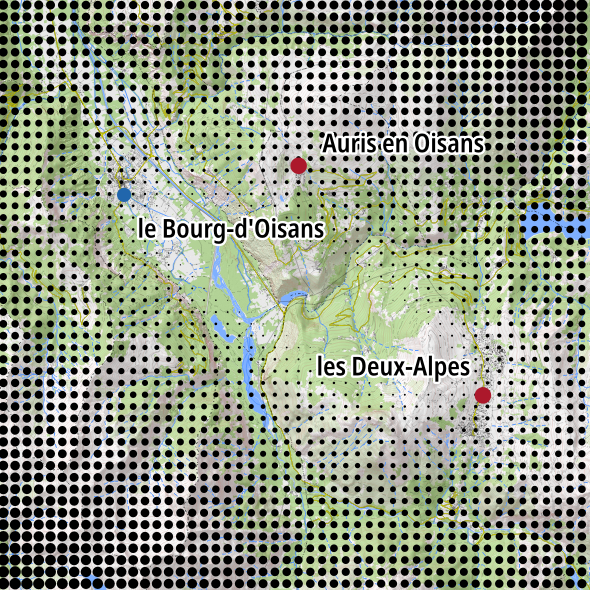
\includegraphics{./figures/EnDirectionDe_metrique_1_FilRouge.png}};
  %
  \begin{scope}
    \node (P2) at ([yshift=-.5cm]image.south east) {};
    \node (P1) at ([yshift=-.5cm]image.south west) {};
    \draw[-] (P2 |- -1cm,-1cm) --++ (-1,0) node[et,pos=.5] {\SI{500}{\meter}}; 
  \end{scope}
\end{tikzpicture}
  \caption{Exemple du calcul de la \emph{métrique}
    \protect\onto{Direction\-De}}
  \label{fig:metrique_direction_de}
\end{figure}

D'autres \emph{métriques,} plus spécifiques (\ie employées par un
petit nombre de \emph{relations de localisation atomiques}) ont
également été développées. C'est par exemple le cas de
\onto{Temps\-De\-Marche} ou \onto{Part\-Visible}, respectivement
utilisées pour la \emph{spatialisation} des \emph{relations de
  localisation} \onto[orla]{Cible\-Voit\-Site} (et son opposée
\onto[orla]{Site\-Voit\-Cible}) et \onto[orla]{A\-Distance\-Temps}
\footnote{Ces trois \emph{relations de localisation atomiques} peuvent
  être utilisées directement. Elles sont par conséquent également
  présentes dans \ac{orl} (\autoref{anx:orl_dic}).}.

La \emph{métrique} \onto{Temps\-De\-Marche} est une \emph{métrique}
extrinsèque, prenant comme paramètre la vitesse moyenne de marche.

La \emph{métrique} \onto{Part\-Visible} est une \emph{métrique}
extrinsèque, non paramétrique.
%
On peut voir une illustration de cette \emph{métrique} sur la
\autoref{fig:metrique_part_lac}. Dans cet exemple la taille du figuré
représente la part de \emph{l'objet de référence} (le lac au centre de
l'image) qui est visible depuis chaque pixel.

\begin{figure}
  \centering
  \begin{tikzpicture}
  \tikzset{et/.style={above,font=\footnotesize\vphantom{Ag}}}
  %
  \node[inner sep=0pt, anchor=south west] (image) at (0,0){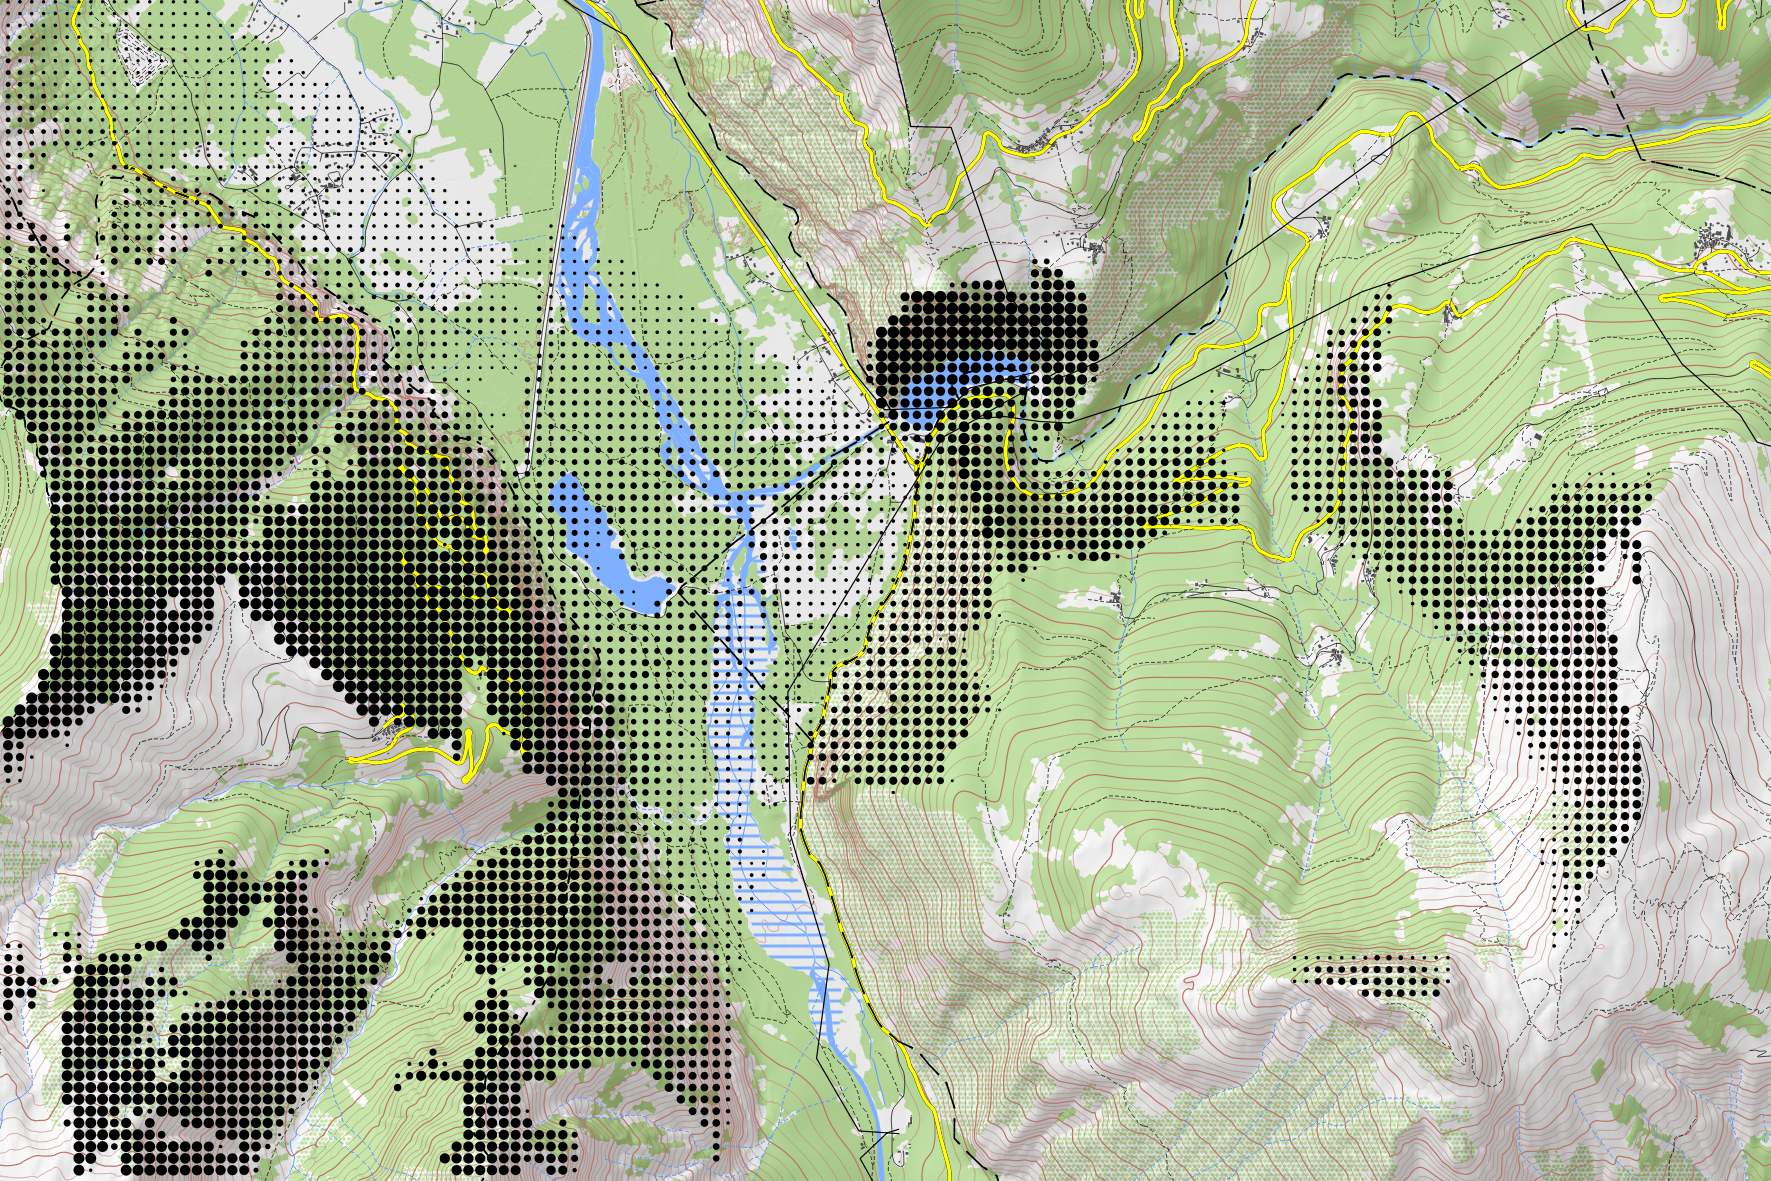
\includegraphics{./figures/Metrique_part_lac_visible.png}};
  %
  \begin{scope}
    \node (P2) at ([yshift=-.5cm]image.south east) {};
    \node (P1) at ([yshift=-.5cm]image.south west) {};
    %
    \foreach \x [evaluate=\xshift using \x/10, evaluate=\rad using (\x * .0004) + .01] in {0,...,100}
    {
      \draw[fill=black,draw=none, below] ([xshift=\xshift cm, yshift=-.5cm]P1) circle [radius=\rad cm];
    }
    %
    \path(P1 |- 0cm,-1cm) --++ (10,0)
    node[et,pos=0] {0}
    node[et,pos=.1] {0,1}
    node[et,pos=.2] {0,2}
    node[et,pos=.3] {0,3}
    node[et,pos=.4] {0,4}
    node[et,pos=.65] {0,65}
    node[et,pos=1] {1};
    % Échelle
    \draw[-] (P2 |- -1cm,-1cm) --++ (-1,0) node[et,pos=.5] {\SI{500}{\meter}};
    % Légende détaillée
    \path (P1) -- (P2) node[pos=.5, yshift=-1cm] {\tiny Pour la légende détaillée du fond topographique voir \autoref{anx:topo_leg}. Sources: BD TOPO 2018, BD ALTI 2018.}; 
  \end{scope}
\end{tikzpicture}
  \caption{Exemple d'une \emph{métrique} issue de la
    \emph{spatialisation} du \emph{fil rouge :} la part de la surface
    visible d'un lac donné.}
  \label{fig:metrique_part_lac}
\end{figure}

%%% Local Variables:
%%% mode: latex
%%% TeX-master: "../../../../main"
%%% End:
